
\begin{figure}
    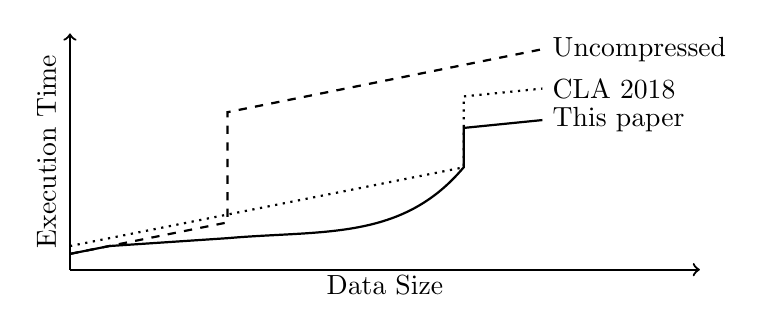
\begin{tikzpicture}

        \draw[->, thick] (0,0) -- (8,0) node[midway, yshift=-0.2cm ]{Data Size};
        \draw[->, thick] (0,0) -- (0,3) node[midway, xshift=-0.3cm,rotate=90]{Execution Time};

        \draw[dashed, thick] (0,0.2) -- (2,0.6) -- (2,2) -- (6,2.8) node[right]{Uncompressed};
        \draw[dotted, thick] (0,0.3) -- (2,0.7) -- (5,1.3) -- (5,2.2) -- (6,2.3) node[right]{CLA 2018};
        \draw[,black,thick] (0,0.2) -- (0.5,0.3) -- (2,0.4) to [out=5,in=-130](5,1.3) -- (5,1.8) -- (6,1.9) node[right]{This paper};
    \end{tikzpicture}
    \caption{Goals of CLA}
    \Description[Goals]{The goals of Compressed Linear Algebra.}
\end{figure}